\documentclass{article}
\usepackage{amsmath}
\usepackage{amssymb}
\usepackage{graphicx}
\usepackage{hyperref}
\usepackage[version=4]{mhchem}

\title{Problem 10}
\date{}

\begin{document}
\maketitle

\section*{Problem}
Four circles of radius \(r\) are mutually tangent inside a circle of radius one unit. Find the radius \(r\). Express your answer in simplified radical form.\\
\centering
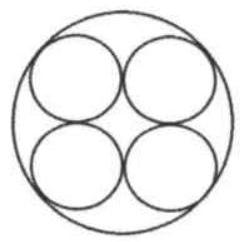
\includegraphics[width=\textwidth]{images/186.jpg}

\section*{Solution}
\(\sqrt{2}-1\).\\
We draw the diameter EF as shown in the figure.\\
Applying Pythagorean Theorem to right triangles \(A D C\) :\\
\((2 r)^{2}+(2 r)^{2}=(2-2 r)^{2} \quad \Rightarrow \quad r=\sqrt{2}-1\).\\
\centering
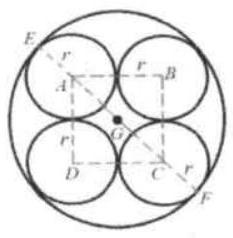
\includegraphics[width=\textwidth]{images/190.jpg}


4. When four points are concyclic, draw the circle.
4.1. Triangles \(A B C\) and \(D B C\) share the side \(B C\). If \(\angle B A C=\angle B D C\), points \(A, B\), \(C\), and \(D\) lie on the same circle.\\
\centering
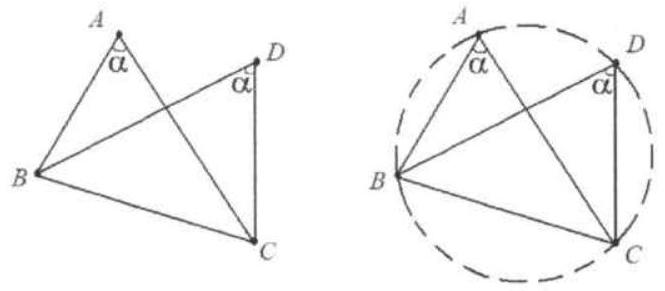
\includegraphics[width=\textwidth]{images/191(3).jpg}\\
4.2. Triangles \(A B C\) and \(A B O\) share the side \(A B\). If \(\angle A O B=2 \angle A C B\), points \(A, B\), \(C\) lie on the same circle \(O\).\\
\centering
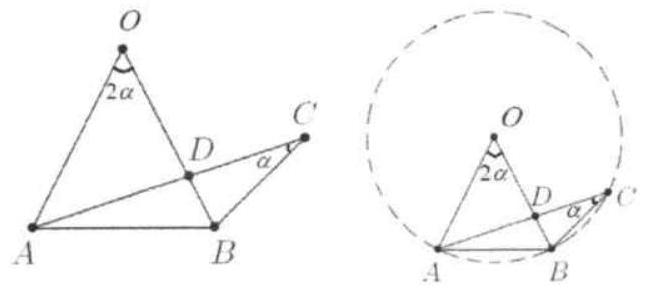
\includegraphics[width=\textwidth]{images/191.jpg}

Theorem 6.10. A quadrilateral is cyclic (i.e. may be inscribed in a circle) if one side subtends congruent angles at the two opposite vertices.

If \(\angle B A C=\angle B D C\), points \(A, B, C\), and \(D\) are concyclic.\\
\centering
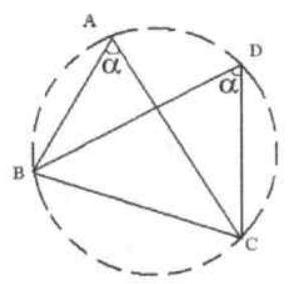
\includegraphics[width=\textwidth]{images/191(2).jpg}

Theorem 6.11. The opposite angles of a cyclic (inscribed) quadrilateral are supplementary.

If the opposite angles of a quadrilateral are supplementary, the quadrilateral can be inscribed by a circle.

If \(\angle B+\angle D=180^{\circ}\), points \(A, B, C\), and \(D\) are concyclic.\\
\centering
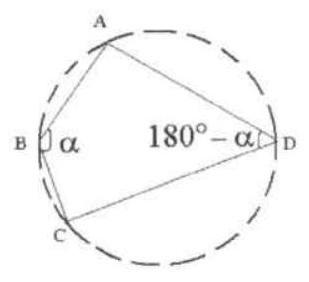
\includegraphics[width=\textwidth]{images/191(1).jpg}


Theorem 6.12. Power of a Point formula (1): If two chords of a circle intersect, the product of the measures of the segments of one chord equals the product of the segments of the other chord.\\
\(P A \times P B=P C \times P D\).

Proof:
Connect \(A C\) and \(B D . \angle P A C=\angle P D B\).\\
\centering

\includegraphics[width=\textwidth]{images/192.jpg}

We know that \(\angle A P C=\angle B P D\). Thus \(\triangle P A C \sim \triangle P D B\).\\
\(\frac{P A}{P C}=\frac{P D}{P B} \quad \Rightarrow P A \cdot P B=P C \cdot P D\).

The converse of Theorem 6.12.
\begin{center}
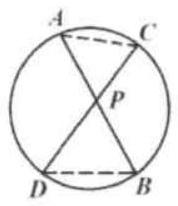
\includegraphics[width=\textwidth]{images/192(1).jpg}
\end{center}

If \(A P \times P B=C P \times P D\), points \(A, C, B\), and \(D\) are concyclic.\\
Theorem 6.13. Power of a Point formula (2): If two secants intersect outside the circle, the product of the measures of one secant and its external segment equals the product of the measures of the other secant and its external segment.\\
\(P A \times P B=P C \times P D\).

Proof:
\begin{center}
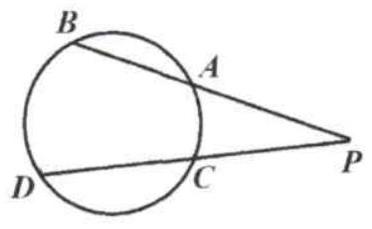
\includegraphics[width=\textwidth]{images/192(3).jpg}
\end{center}

Connect \(A C\) and \(B D . \angle P A C=\angle P D B\).\\
We know that \(\angle A P C=\angle B P D\). Thus \(\triangle P A C \sim \triangle P D B\).\\
\(\frac{P A}{P C}=\frac{P D}{P B} \quad \Rightarrow P A \cdot P B=P C \cdot P D\).\\
\centering
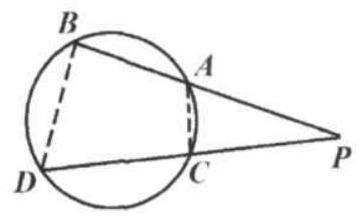
\includegraphics[width=\textwidth]{images/192(2).jpg}

The converse of Theorem 6.13.
If \(P A \cdot P B=P C \cdot P D\), points \(A, B, D\), and \(C\) are concyclic.\\
Theorem 6.14. Power of a Point formula (3): \(P C^{2}=P B \times P A\)\\
\centering
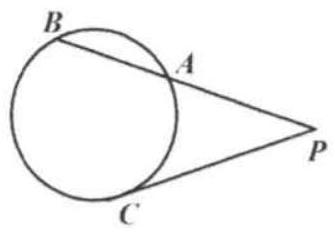
\includegraphics[width=\textwidth]{images/192(4).jpg}


Proof:
Connect \(A C\) and \(B C . \angle P C A=\angle P B C\) (both face the same arc \(A C\) ). We know that \(\angle A P C=\angle B P C\). Thus, \(\triangle P A C \sim \triangle P C B\).\\
\(\frac{P A}{P C}=\frac{P C}{P B} \quad \Rightarrow P C^{2}=P A \times P B\)\\
\centering
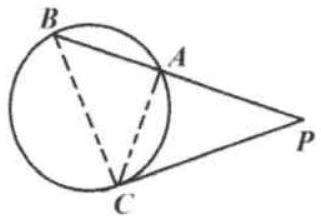
\includegraphics[width=\textwidth]{images/193.jpg}

Theorem 6.15. Ptolemy's Theorem: If quadrilateral \(A B C D\) is a cyclic quadrilateral, then \(A C \times B D=A B \times C D+A D \times B C\).

Proof:
Method 1:\\
Extend \(A B\) to \(P\) such that \(\angle P C A=\angle D C B\).\\
Then \(\triangle A C P \sim \triangle D C B . \frac{A C}{C D}=\frac{A P}{B D}\).\\
\centering
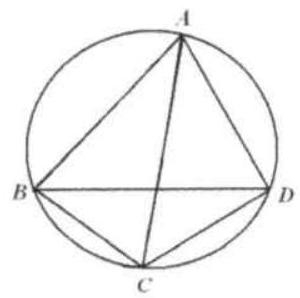
\includegraphics[width=\textwidth]{images/193(2).jpg}

So \(A C \cdot B D=C D \cdot A P\)\\
We also have \(\angle C B P=\angle A D C, \angle B P C=\angle C B D=\angle C A D\).\\
Then \(\triangle A C D \sim \triangle P C B\). We have \(\frac{A D}{P B}=\frac{C D}{B C}\) or\\
\(A D \cdot B C=C D \cdot P B\)\\
(1) - (2): \(A C \cdot B D-A D \cdot B C=C D(A P-P B)=A B \cdot C D\).\\
\centering
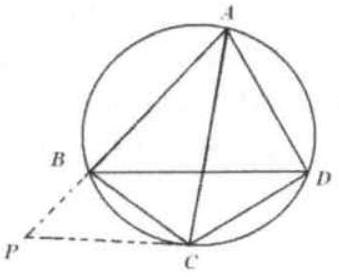
\includegraphics[width=\textwidth]{images/193(1).jpg}

That is, \(A C \cdot B D=A B \cdot C D+B C \cdot A D\).

\end{document}
